\documentclass[a4paper]{article}

\usepackage[utf8]{inputenc}
\usepackage[T1]{fontenc}
\usepackage{libertine}
\usepackage[french]{babel}
\usepackage{amsmath}
\usepackage{xcolor}
\usepackage{graphicx}
\usepackage{listings}
\usepackage{caption}
\usepackage{wrapfig}
\usepackage{float}

\DeclareGraphicsExtensions{.png, .jpeg, .jpg, .svg}

\title{Faster Text Fingerprinting}
\author{Hugo \textsc{Mougard} et Soufian \textsc{Salim}}
\date{\today}

\begin{document}

\maketitle

\section{Introduction}

\subsection{Qu'est ce qu'un \emph{fingerprint} ?}

Pour $s = s_{1} .. s_{n}$ un texte sur un alphabet $\Sigma$, un \textit{fingerprint} $f$ est un ensemble des caractères distincts contenus dans l'une de ses sous-chaînes. Le \emph{fingerprinting} consiste à calculer l'ensemble $\mathcal{F}$ de tous les \emph{fingerprints} $f$ de toutes les sous-chaines de $s$.  \newline

Par exemple, pour la chaîne $s = a_{1} b_{2} c_{3} a_{4} a_{5} d_{6} d_{7} b_{8}$, le \emph{fingerprint} de $[3,7]$ est $\{cad\}$. \newline

Le \emph{fingerprinting} d'un texte $s$ c'est le calcul de tous les $f$ de $\mathcal{F}$.

\subsection{Applications possibles}

Les fingerprints sont utiles quand l'on souhaite travailler sur des ensembles de caractéristiques plutôt que des séquences de caractéristiques. On peut dire que les \emph{fingerprints} sont aux ensembles ce que les n-grams sont aux séquences. En bioinformatique, les \emph{fingerprints} sont utilisés pour la recherche approchée de chaîne de caractères. En traitement des langues, ils sont utilisés pour l'apprentissage de distributions ensemblistes \cite{amir}. Par exemple, pour un classificateur entraîné pour désambiguiser les mots, on pourrait apprendre la distribution des \emph{fingerprints} dans des patrons donnés : \newline

\emph{It might be a \{Adj, Adv\} match.}

\subsection{Problèmes soulevés}

\begin{itemize}
	\item Calculer l'ensemble $\mathcal{F}$ des \emph{fingerprints}
	\item Déterminer si un \emph{fingerprint} $f$ est dans $\mathcal{F}$
	\item Retrouver les occurrences de $f$ dans $s$
	\item Calculer le nombre de \emph{fingerprints} de taille $k$ dans $s$
	\item ...
\end{itemize}

Cet article s'intéresse principalement au premier de ces problèmes : calculer l'ensemble $\mathcal{F}$ des \emph{fingerprints}.

\subsection{Avant de commencer}

Deux notions importantes sont à connaître avant de comprendre l'apport de l'article sur le problème du calcul de $\mathcal{F}$ :

\begin{itemize}
	\item Les localisations maximales
	\item Les copies et les classes d'équivalence
\end{itemize}

\subsubsection{Localisations maximales}

On note $\mathcal{C}$ un ensemble de lettres de $\Sigma$. Une location maximale de $\mathcal{C}$ dans $s$ est un intervalle $[i,j]$ tel que : \newline
		
\begin{itemize}
	\item $\mathcal{C}_{s}(i,j) = \mathcal{C}$
	\item Si $i > 1$, $s_{i-1} \notin$ $\mathcal{C}_{s}(i,j)$
	\item Si $j < n$, $s_{j+1} \notin$ $\mathcal{C}_{s}(i,j)$
\end{itemize}

On note $\mathcal{L}$ l'ensemble des locations maximales de tous les \textit{fingerprints} de $\mathcal{F}$. \newline

Par exemple, pour la chaîne $s = a_{1} b_{2} c_{3} a_{4} a_{5} d_{6} d_{7} b_{8}$, la seule location maximale de $abc$ est $\langle1,5\rangle$.

\subsubsection{Copies et classes d'équivalence}

Deux locations maximales $\langle i,j \rangle$ et $\langle k,l \rangle$ de $s$ sont des copies si $s_{i}..s_{j} = s_{k}..s_{l}$. On note $\mathcal{L}_{\mathcal{C}}$ l'ensemble des classes d'équivalence. \newline

Par exemple, pour la chaîne $s = a_{1} b_{2} a_{3} d_{4} a_{5} b_{6} a_{7}$, $\langle1,3\rangle$ et $\langle5,7\rangle$ sont des copies.

\subsection{Contexte}

Pour le calcul de la complexité, il faut noter que $|\mathcal{F}| \leq |\mathcal{L}_{\mathcal{C}}| \leq |\mathcal{L}|$.

\begin{enumerate}
	\item Efficient Text Fingerprinting via Parikh Mapping (2003) \newline
$\rightarrow \mathcal{O}(n|\Sigma|$ $log$ $n$ $log$ $|\Sigma|)$
	\item New Algorithms for Text Fingerprinting (2006) \newline
$\rightarrow \mathcal{O}(n + |\mathcal{L}|$ $log$ $|\Sigma|)$
	\item Faster Text Fingerprinting (2008) \newline
$\rightarrow \mathcal{O}((n + |\mathcal{L}_{\mathcal{C}})|$ $log$ $|\Sigma|)$
	\item Various Improvements to Text Fingerprinting (2013) \newline
$\rightarrow \mathcal{O}(n + |\mathcal{L}|)$ (Approximatif - \emph{Monte-Carlo})
\end{enumerate}

\subsection{Apports de l'article}

Dans les approches antérieures, les \emph{fingerprints} dans une liste, ce qui entraînait des redondances dans les calculs. Ici, les \emph{fingerprints} sont organisés dans un arbre, et on ne retrouve pas cette redondance.

\subsection{Vue d'ensemble}
	
\begin{enumerate}
	\item Construire l'arbre des suffixes de $s$
	\item À partir de l'arbre des suffixes, construire un arbre des participations
	\item À partir de l'arbre des participations, nommer tous les \textit{fingerprints} de $s$
\end{enumerate}

\section{\textit{Participation Tree}}

\begin{enumerate}
	\item On le note $PT$
	\item Il est construit à partir de l'arbre des suffixes (noté $ST$) de $s$
	\item Il contient l'ensemble des \emph{fingerprints} $f$ de $\mathcal{F}$
\end{enumerate}

\subsection{Construction de l'arbre}

Exemple de construction de l'arbre pour la chaîne $ataltatlt\#$ :

\subsubsection{Étape 1}

\begin{figure}[H]
\centering
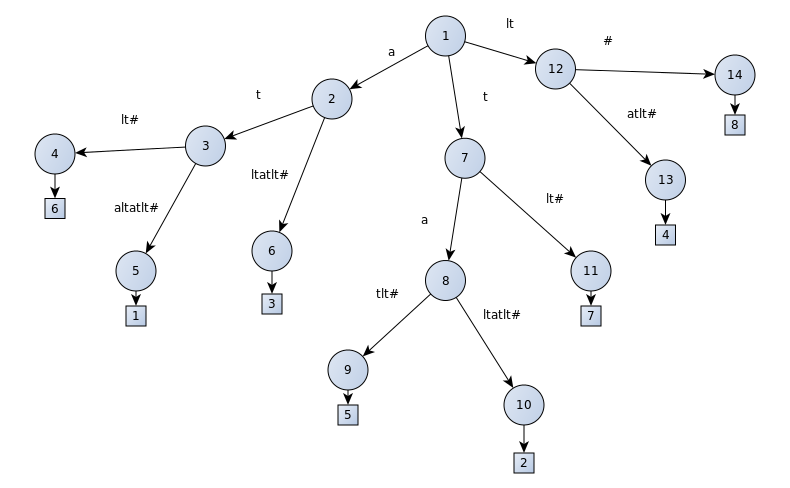
\includegraphics[width=80mm]{./slides/img/construction-0.png}
\caption{État initial : l'arbre des suffixes}
\label{overflow}
\end{figure}

\subsubsection{Étape 2}

\begin{figure}[H]
\centering
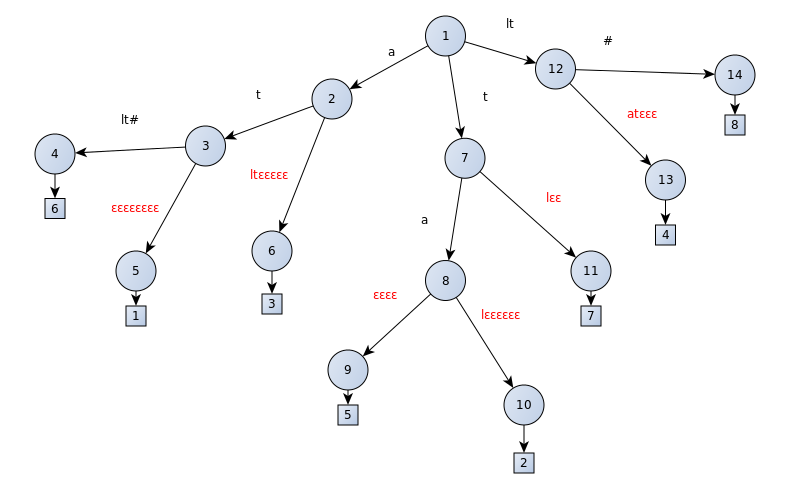
\includegraphics[width=80mm]{./slides/img/construction-1.png}
\caption{On réduit tous les caractères à partir de la seconde occurrence du premier caractère du chemin à $\varepsilon$}
\label{overflow}
\end{figure}

\subsubsection{Étape 3}

\begin{figure}[H]
\centering
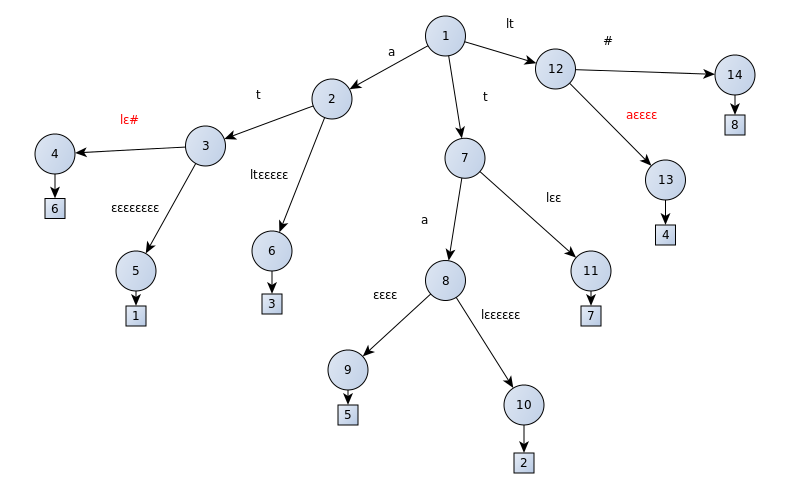
\includegraphics[width=80mm]{./slides/img/construction-2.png}
\caption{De la racine au dernier caractère avant $\varepsilon$, on ne garde que la première occurrence de chaque caractère.}
\label{overflow}
\end{figure}

\subsubsection{Étape 4}

\begin{figure}[H]
\centering
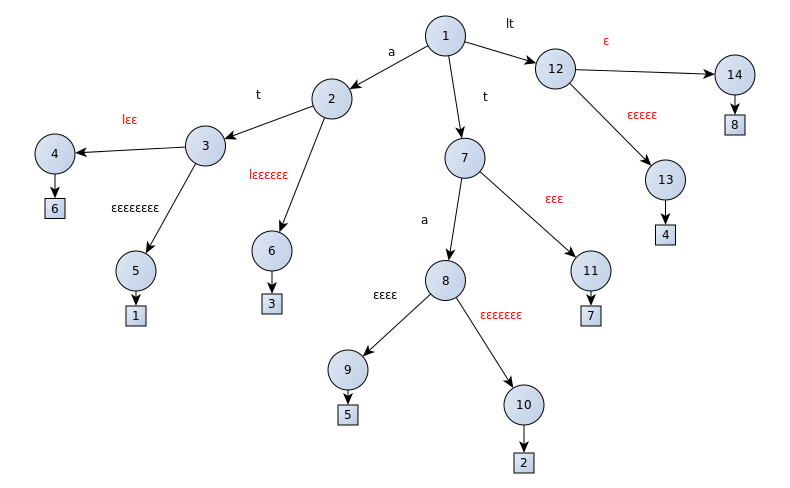
\includegraphics[width=80mm]{./slides/img/construction-3.png}
\caption{On remplace le dernier caractère de chaque chemin de la racine à une feuille par $\varepsilon$}
\label{overflow}
\end{figure}

\subsubsection{Étape 5}

\begin{figure}[H]
\centering
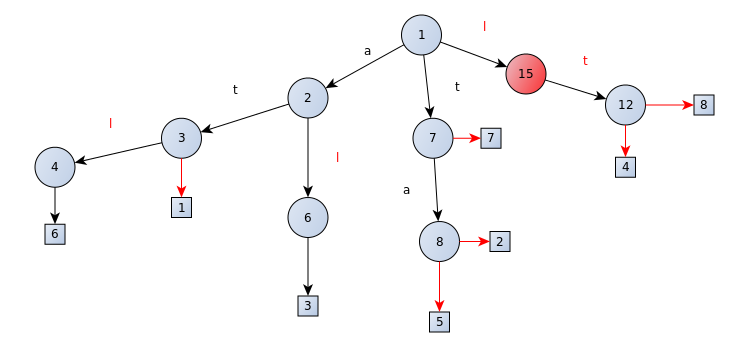
\includegraphics[width=80mm]{./slides/img/construction-45.png}
\caption{On déploie l'arbre et on supprime les branches vides}
\label{overflow}
\end{figure}

\subsection{Théorème}

$\Phi$ étant définie comme une fonction retournant l'ensemble des localisations maximales correspondant à un chemin $z$ de $PT$, \newline

\textbf{toutes les localisations maximales sont dans l'image $\Phi(z)$ d'un chemin $z$ dans $PT(s = s_{1}..s_{n})$, et la taille de $PT(s)$ est $\mathcal{O}(|\mathcal{L}_{\mathcal{C}}|)$}.

\subsection{Du \emph{Suffix} Tree au \emph{Participation Tree}}

Les principes de l'algorithme sont les suivants : calculer les participations des branches aux fingerprints les unes après les autres, marquer les arêtes calculées pour ne pas les recalculer, et calculer seulement les deltas des valeurs nécessaires à chaque pas.

\subsubsection{Algorithme efficace}

\textbf{Pour chaque branche}

$\rightarrow$ Calculer la chaîne indicée $poc_i$ des premières occurrences de chaque caractère de la chaîne sur la branche

$\rightarrow$ Calculer la position $p_i$ de l'occurrence suivante du premier caractère de la branche

\textbf{Pour chaque arête $[x,y]$ sur la branche, de la feuille à la racine}

$\rightarrow$ Retourner la sous chaîne de $poc_i$ allant de l'indice $l$ à l'indice $r$ avec $argmin_l(l \leq x)$ et $argmax_r(r < p \land r \leq y)$. Peut valoir $\varepsilon$.

\subsubsection{Astuces algorithmiques}

Représentation des "chaque première occurrence" dans un arbre AVL
Stockage des positions des caractères dans des listes pour pouvoir calculer l'itération suivante depuis l'itération courante en $\mathcal{O}(log |\Sigma|)$. \newline

$\rightarrow$ $\mathcal{O}(n \times log |\Sigma| + |\mathcal{L}_\mathcal{c}|)$ en temps.

\section{Nommage des \emph{fingerprints}}

\paragraph{Pourquoi donner un nom aux \emph{fingerprints} ?} Pour
rendre la gestion des fingerprints plus aisée \cite{amir, karp}. Par gestio nous entendons

\subsection{Nommage hiérarchique}

\subsection{Utiliser les deltas de participation entre \emph{fingerprints}}

\subsection{Nommage d'une liste de listes de participations}

\subsection{Nommage sur l'arbre}

\section{Conclusion}

L'article propose une méthode de calcul de $\mathcal{F}$ basée sur l'arbre des suffixes. Il adapte une fonction de nommage existante, originellement appliquée à une liste, à une structure arborescente : l'arbre des participations. La méthode proposée est état de l'art pour la complexité dans le pire des cas d'une construction exacte. \newline

En conservant le mapping des noms et les noms des fingerprints obtenues, il est facile de répondre aux questions posées dans l'introduction :\newline

\begin{itemize}
	\item Trouver le nombre de fingerprints \newline $\rightarrow$ Autant de fingerprints qu'il y a de noms.
	\item Déterminer si un fingerprint est dans F \newline $\rightarrow$ Nommer le fingerprint et regarder si le nom est dans l'ensemble des noms calculé. \newline
\end{itemize} 

\bibliography{biblio.bib}
\bibliographystyle{amsalpha}

\end{document}